
\section{The Theory that would not die: Bayesian Probability}


\noindent
What do guiding NASA's \textbf{Apollo 11} mission to the lunar surface (\textit{July 1969}) \cite{schmidt1966application}, locating the lost wreckage of \textbf{Air France Flight 447} in the Atlantic (\textit{May 2011}) \cite{stone2014search, cornell2015bayes}, and \textbf{Google DeepMind's AlphaGo} defeating world champion Lee Sedol (\textit{March 2016}) \cite{silver2016mastering} all have in common? 

The answer lies in \textbf{Bayesian statistics}. Despite spanning different eras and domains, each historic breakthrough relied on updating probabilistic beliefs in real time under extreme uncertainty. This chapter explores the history of Bayesian inference, tracing how an 18th-century theorem evolved into one of the most powerful computational tools in modern applied mathematics.


\subsection{Was Bayes trying to calculate the existence of God in the 18th century?}
In the eighteenth century, Thomas Bayes began developing what would later become Bayes' theorem, although his work remained unpublished during his lifetime. After Bayes' death in 1761, his friend Richard Price discovered the manuscript among his papers, edited it, and presented it to the Royal Society in 1763 under the title An Essay towards Solving a Problem in the Doctrine of Chances. Price recognised that Bayes' mathematical framework had important philosophical implications and used it to support arguments about reasoning under uncertainty.

\fcolorbox{red}{red!10}{
  \textcolor{red}{\textbf{TODO: Add an image of the Bayes pool table experiment or the square picture CAN BE ADDED LATER IN section 7.3.}}
}

One popular historical interpretation is that Bayes originally developed his theorem in response to David Hume's 1748 essay Of Miracles. Hume argued that miracles are so improbable that no amount of human testimony could rationally justify believing they had occurred. According to this interpretation, Bayes sought to show mathematically that sufficiently strong accumulated evidence could outweigh the initial improbability of an event, providing a rational framework for evaluating extraordinary claims such as miracles, divine providence, or the resurrection of Jesus Christ. Richard Price later strengthened this connection by explicitly applying Bayesian reasoning in defence of religious belief after Bayes' death (Stigler, 1986).
The English Enlightenment period was when academicians, philosiphers, mathematicians attempted to quantify philosophical ideas. Many statistical and logical frameworks emerged from time as a result of these motivations. 

However, this interpretation remains debated. McGrayne (2011) argues that there is no direct evidence that Bayes intended his work as a response to Hume. Bayes left few personal writings explaining his motivations, making it difficult to determine his original purpose. Some historians instead suggest that Bayes was simply interested in solving a mathematical problem concerning inverse probability, with Price later recognising its wider philosophical and theological significance. In this view, the association between Bayes' theorem and Hume's essay is largely the result of Price's interpretation rather than Bayes' own intentions.

\begin{figure}
    \centering
    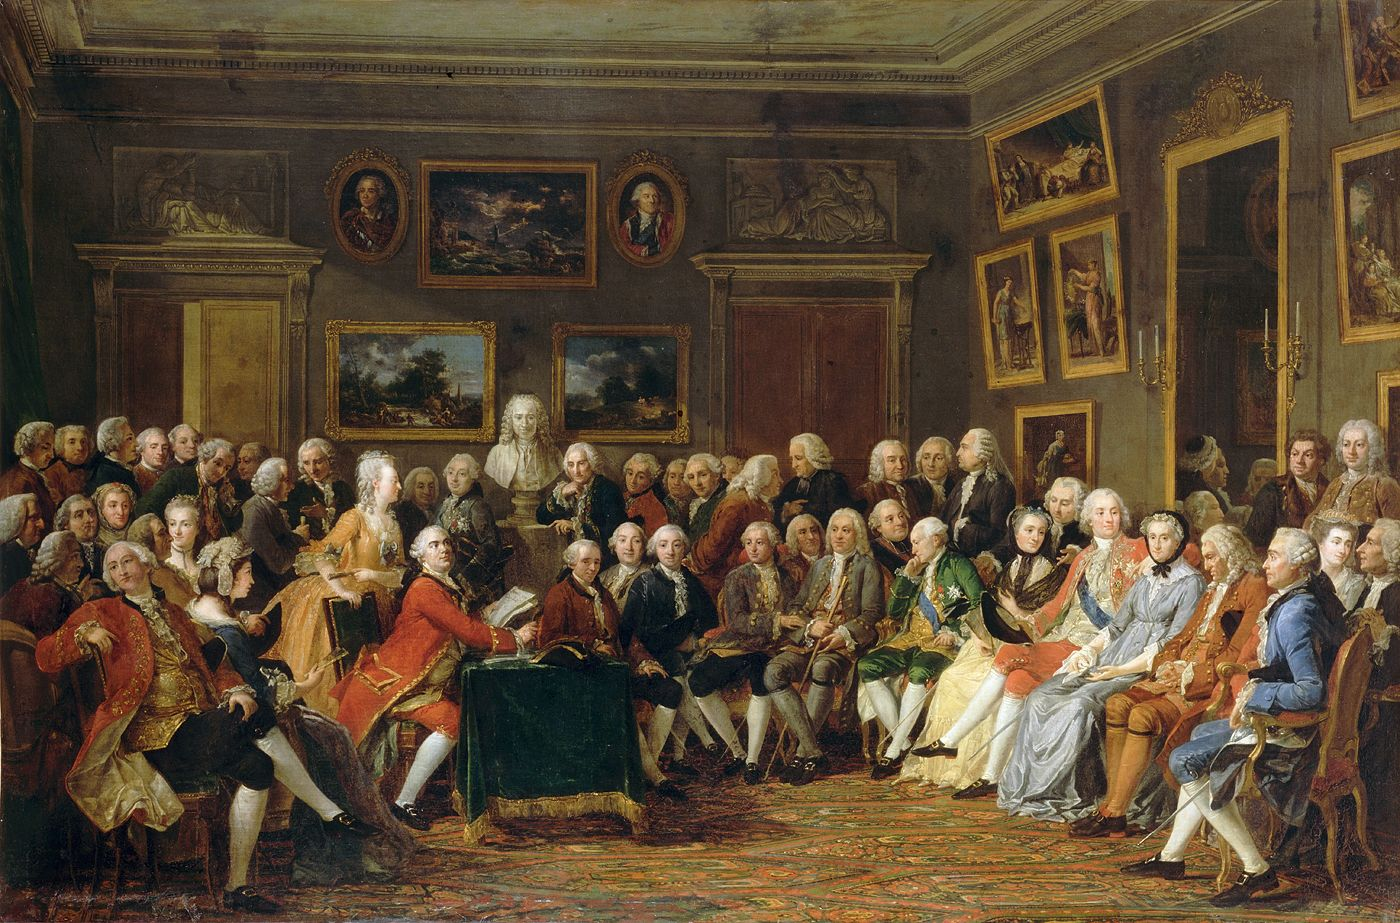
\includegraphics[width=0.75\linewidth]{Les_salons_au_XVIIIe_siècle_-_Histoire_Image.jpg}
    \caption{Enlightenment Period Painting "In the Salon of Madame Geoffrin in 1755."}
    \label{fig:placeholder}
\end{figure}


Regardless of Bayes' original motivation, his work emerged during the English Enlightenment, a period in which philosophers, mathematicians, and scientists increasingly sought to describe uncertainty and rational belief using mathematics. This intellectual movement produced many of the statistical and logical ideas that would later become the foundations of modern probability theory and Bayesian statistics.


%\fcolorbox{red}{red!10}{
 % \textcolor{red}{\textbf{TODO: Add an image of the Enlightenment period.}}
%}

\subsection*{REFERENCES TO BE COMPILED}
McGrayne, S. B. (2011). The Theory That Would Not Die: How Bayes' Rule Cracked the Enigma Code, Hunted Down Russian Submarines, and Emerged Triumphant from Two Centuries of Controversy. Yale University Press.

Stigler, S. M. (1986). The History of Statistics: The Measurement of Uncertainty Before 1900. Harvard University Press.

Hummes book also mentined An Enquiry Concerning Human Understanding



%Short answer is: No.

%But there are stereotypes that Bayes, or more specifically Price, connected the theory with religion - to defend Christian theology as a direct, "more intellectual and rigourous" way to counteract the Scottish Enlightenment philosopher David Hume. (For context: English enlightenment period: from the late 17th century to the late 18th century (roughly 1685 to 1815).

%Bayes instructed his assistance to place a ball in an unknown position on the snooker table and Bayes would throw balls behind his head on the table. The assistant would  then only announce whether the balls landed to the left or to the right of the placed ball. Using this new information bayes would try to predict the where the ball was placed.


\subsection{Laplace's independent search for laws of nature hidden in astronomy data}
By the late eighteenth century, astronomers had collected hundreds of years of observations on the motions of planets such as Jupiter and Saturn. While this gave scientists a huge amount of data to work with, much of it contained observational mistakes, recording errors, and inconsistencies. These errors made it seem as though the planets did not always follow Newton's laws of motion. Instead of assuming Newton's theory was wrong, Pierre Simon Laplace (1749–1827) looked for a way to separate the true motion of the planets from errors in the data.

INCLUSE THE THEORY BEFORE THAT JUPITER AND SATURN WOULD CRASH INTO EACH OTHER

Although Thomas Bayes first introduced the theorem that is now named after him, it was Laplace who independently developed and mathematically formalised the theory. His work was much more rigorous and widely recognised, which is why some historians argue that it should really be known as the Bayes–Laplace theorem.

REFERENCE 
Stigler, S. M. (1986). The history of statistics: The measurement of uncertainty before 1900. Harvard University Press.

Laplace's main contribution was what became known as inverse probability. Traditional or forward modelling asks, "If this model is correct, what data should we observe?" Laplace turned this around and instead asked, "Given all of this observed data, what model most likely produced it, what are the model parameters, and how certain can we be about them?" This was a major shift because it focused on learning from data instead of simply testing a model.


\fcolorbox{red}{red!10}{
  \textcolor{red}{\textbf{TODO: Add an image of the Laplace theorem found in google images CHECK IF EVE HAS ANY PICs.}}
}

His approach helped explain that many of the differences between observations and Newton's predictions were due to measurement errors rather than problems with the laws of physics. This idea became the foundation of Bayesian inference, which is still widely used today in statistics, machine learning, and many areas of scientific research.


Found link similar to what we are working on 
McGrayne, S. B. (2011). The theory that would not die: How Bayes' rule cracked the enigma code, hunted down Russian submarines, and emerged triumphant from two centuries of controversy. Yale University Press.

Laplace, P.-S. (1774). Mémoire sur la probabilité des causes par les événements. Mémoires de l'Académie Royale des Sciences de Paris. (This is Laplace's first publication introducing inverse probability.)

%Laplace formalised the rigourous mathematical proof of bayes
%The birth of "inverse probability" -- note Laplace was very famous and a rigourous mathematician compared to bayes and price. He formulated the theory mathematically, and some even beleive the theory should be named after him. 

%The initial problems with big data he was strugging to work with - centuries of data aggregation and messy data of the orbits of Jupyter and Saturn --> many mistakes led to misalignment with Newton's laws of motion --> Laplace solved the human error (and other errors) through finding inverse probability. 

%Forward modelling asks: "Given this model, what does out data look like?"

%Laplace asked: " Given i have all this data, what does my model look like? what are my model parameters and what is the probability of uncertainty that these parameters are true?"

\subsection{So what is Bayes' theorem?} 

The previous sections introduced the historical origins of Bayesian reasoning through the work of Thomas Bayes and Pierre-Simon Laplace. However, the theorem itself is often presented as a mathematical formula without explaining the intuition behind it. 
MAYBE CHANGE WHST YOU WROTE
In reality, Bayes' theorem is simply a rule for updating probabilities when new information becomes available. Rather than treating probability as fixed, Bayesian inference allows beliefs to change as evidence accumulates.

Before introducing Bayes' theorem, it is first necessary to understand the concept of conditional probability.

Conditional probability measures the probability of an event occurring given that another event has already occurred. Suppose two events, (A) and (B), are defined. The conditional probability of event (A) occurring given that event (B) has occurred is written as (P(A|B)) and is defined as
\begin{equation}
[
P(A|B)=\frac{P(A\cap B)}{P(B)}.
]
\end{equation}

This definition states that once event (B) has occurred, the original sample space is restricted only to outcomes contained within (B). The probability of (A) must further be recalculated within this reduced set of possibilities.

The same joint probability may also be written in the opposite direction,
\begin{equation}
[
P(B|A)=\frac{P(A\cap B)}{P(A)}.
]
\end{equation}

Since both equations describe the same joint event (P(A|B)), they can be equated,
\begin{equation}
[ 
P(A|B)P(B)=P(B|A)P(A),
]
\end{equation}
which, after rearranging, gives Bayes' theorem,
\begin{equation}
    [P(A|B)=\frac{P(B|A)P(A)}{P(B)}.]
\end{equation}

The theorem contains four quantities, each with a seperate interpretation:
\begin{itemize}
    \item \textbf{Prior probability (P(A)):} the initial belief about an event before observing new evidence.
\end{itemize}   
\begin{itemize}
    \item \textbf{Likelihood (P(B|A)):} the probability of observing the evidence assuming the hypothesis is true.
\end{itemize}   
\begin{itemize}
    \item \textbf{Evidence (P(B)):} the overall probability of observing the evidence.
\end{itemize}
\begin{itemize}
    \item \textbf{Posterior probability (P(A|B)):} the updated belief after incorporating the evidence.
\end{itemize}

To summarise, rather than introducing a completely new probability, Bayes' theorem simply redistributes existing probabilities using newly acquired information. This process of continually updating beliefs is known as Bayesian inference.
\subsubsection{A geometric interpretation}

Although Bayes' theorem is usually introduced algebraically, it is often easier to understand geometrically. Imagine a rectangle representing an entire population. The width of the rectangle corresponds to the prior probability (P(A)), while the remaining width represents the complement of the event. The rectangle is then divided horizontally according to whether the observed evidence occurs. The overlapping region corresponds to the joint probability $(P(A\cap B)).$

\fcolorbox{red}{red!10}{
  \textcolor{red}{\textbf{TODO: Add an image of the Geometric interpretation of Bayes' theorem showing prior probability, likelihood and posterior probability}}
}

Viewed geometrically, Bayes' theorem asks a remarkably simple question:
\begin{quote}
    Of all the individuals for whom the evidence is true, what proportion actually belong to the hypothesis being investigated?
\end{quote}

Consequently, the posterior probability is obtained by dividing the area of the overlap by the total area representing the observed evidence. This geometric perspective illustrates that Bayes' theorem is not merely an algebraic identity but a natural consequence of partitioning probability space.

\subsubsection{The Medical paradox}
One of the most famous demonstrations of Bayes' theorem is the medical testing paradox. It highlights why intuitive reasoning about probabilities often leads to incorrect conclusions.

Suppose a disease affects only 1\% of the population. A medical test correctly identifies an infected patient 99\% of the time (99\% sensitivity) and correctly identifies a healthy patient 95\% of the time (95\% specificity).

Many people assume that receiving a positive test result means there is approximately a 99\% chance they have the disease. Bayes' theorem shows that this conclusion is incorrect because it ignores the rarity of the disease.

\fcolorbox{red}{red!10}{%
  \parbox{\dimexpr\linewidth-2\fboxsep-2\fboxrule\relax}{%
    \raggedright
    \textcolor{black}{%  
      \begin{enumerate}
        \itembf To illustrate this, imagine testing 10,000 people.
        \item Approximately 100 people genuinely have the disease.
        \item The test correctly identifies 99 of these individuals.
        \item The remaining 9,900 people are healthy.
        Since the false positive rate is 5\%, approximately 495 healthy people will also receive a positive result.
      \end{enumerate}
    }%
  }%
}%

Therefore, there are
\begin{equation}
    99+495=594    
\end{equation}

positive test results in total, yet only 99 correspond to genuine cases.
The probability that a person actually has the disease after receiving a positive result is therefore

$\frac{99}{594}$
$\approx0.167.$

In other words, despite the test appearing highly accurate, the probability that a positive result indicates genuine disease is only about 16.7\%. The overwhelming number of healthy individuals means that false positives dominate the positive test results.


\fcolorbox{red}{red!10}{
  \textcolor{red}{\textbf{TODO: Add an image of a Frequency tree about the medical testing paradox}}}

This phenomenon demonstrates one of the most important principles of Bayesian inference: evidence cannot be interpreted in isolation.
The strength of new evidence depends critically on the prior probability of the event under investigation. 
Ignoring the prior often leads to serious errors in judgement, a mistake known as the base-rate fallacy.
Bayes' theorem therefore provides much more than a mathematical identity.
It offers a principled framework for learning from evidence by continuously refining beliefs as additional information becomes available. 
This seemingly simple idea would later become the mathematical foundation of modern Bayesian statistics, probabilistic machine learning, artificial intelligence, medical diagnosis, robotics, and countless other applications explored throughout the remainder of this chapter.

NEED HELP WITH THE ALIGNMENT
%Here was explain the theorem in practice with simple examples from : 
%Explain conditional probability then bayes theorem GEOMETRICALLY

%https://www.3blue1brown.com/lessons/bayes-theorem/ 
%+ Proof
%https://youtu.be/U_85TaXbeIo?si=B8yTYpSsGEeVEBOe 
%The medical test paradox, and redesigning Bayes' rule: USE IMAGES
%https://youtu.be/lG4VkPoG3ko?si=jxpWbi86mc0MeRBM


\subsection{Bayesian developments after 1950's} 
Despite strong criticism from Ronald Fisher and many frequentist statisticians, Bayesian statistics continued to develop throughout the twentieth century. Frequentists argued that probability should only describe long run frequencies of repeated events and rejected the idea of assigning probabilities to unknown parameters. However, Bayesian researchers believed probability could also represent uncertainty about unknown quantities, allowing prior knowledge to be combined with observed data. By the 1950s, this debate had led to two major branches of Bayesian statistics: Bayesian inference and Bayesian decision theory.

Bayesian inference focused on updating beliefs using Bayes' theorem. Starting with a prior distribution, new evidence is incorporated through the likelihood function to produce a posterior distribution, representing updated beliefs about the unknown parameters. During this period, Harold Jeffreys made important contributions by introducing objective Bayesian methods. His most well known contribution, Jeffreys prior, provided a way of choosing non-informative priors using the Fisher information matrix, allowing Bayesian analyses to be performed with minimal subjective assumptions. Alongside this, statisticians continued to investigate different choices of informative and non-informative priors, including the uniform prior originally suggested by Laplace.
%(Jeffreys, 1939)

At the same time, Bayesian decision theory developed alongside advances in statistical decision theory. Abraham Wald established the mathematical foundations of decision theory during the 1940s while working on military problems for the United States during the Second World War. One of the famous examples was the aircraft survival problem, where Wald demonstrated that armour should be placed where returning aircraft showed the least damage, since aircraft hit in those locations were less likely to survive. His work introduced the concept of minimising expected loss when making decisions under uncertainty. 
%(Wald, 1950).
article: https://medium.com/@penguinpress/an-excerpt-from-how-not-to-be-wrong-by-jordan-ellenberg-664e708cfc3d

\begin{figure}
    \centering
    
\includegraphics[width=0.4\linewidth]{images.jpeg}
    \caption{Aircraft Survivability Diagram}
    \label{fig:placeholder}
\end{figure}



Leonard J. Savage later combined Wald's statistical decision framework with Bayesian probability. In The Foundations of Statistics (1954), Savage argued that rational decisions should be based on posterior probabilities together with a utility or loss function. Rather than selecting the most likely outcome alone, Bayesian decision theory chooses the action that minimises expected loss or maximises expected utility. This framework closely links to utility theory and provides a practical extension of Bayesian inference from estimating unknown quantities to making optimal decisions.


Today, these two branches are rarely separated. Modern Bayesian methods first use inference to estimate a posterior distribution and then apply decision theory to determine the optimal action. This combination forms the basis of many artificial intelligence and machine learning systems, where posterior distributions quantify uncertainty while loss functions guide decision making. Applications now span medicine, economics, robotics, autonomous systems, and natural language processing, demonstrating how Bayesian inference and Bayesian decision theory together provide a principled framework for learning from data and making decisions under uncertainty.


These developments also laid the foundations for probabilistic reasoning in computing. During the 1930s, Alan Turing studied at Princeton University, where he became acquainted with John von Neumann, whose work on computing and game theory would later complement Bayesian ideas about rational decision making. At the same time, Turing was familiar with Harold Jeffreys' work on probability, and these ideas would later influence his approach to reasoning under uncertainty during the Second World War. This connection provides a natural transition from the theoretical development of Bayesian statistics to one of its earliest practical applications: Turing's Bayesian methods for breaking the German Enigma cipher at Bletchley Park.

CHECK WITH IVE IF ANY INFO IS REPEATED


%Bayesian methods contiued to be developed and attempted to be enhanced regardless of Fishers and other frequentist statisticians protests and refusal to acknowledge the concepts. 
%In the 1950's, 2 branches of bayes were developed. Bayesian inference and bayesian Decision theory. -> Both of which were later combined to make optimal decisions in modern bayesian applications like, economics, medicine and more.

%Looking specifically at Bayesian Decision Theory Branch 1:
%Wald worked with the US on aircraft armors where he used the general stats decision theory. - Aircraft survival experiment
%Savage in 1970's worked on formal bayesian statistical decsion theory

%Decision theory - bayes risk function vs frequentist risk. Link to utility theory example in LLN and CLT chapters. 
%Modern AI systems use both branches- Bayesian inference + Posterior distribution + Decision theory (Loss functions, Expected utility) = optimal decision making

%Branch 2:
%Jefferies prior - Fisher info matrix
%Laplace prior? Informative and non-informative?
%Work  that ties to Alan Turing's work


%% ------------------------------------------
%% ------------------------------------------
% \subsection{Alan Turing and Joan Clarke: Breaking the Enigma}

% Alan turing and von neumann -- alan rivarly 

% jeffrey and Neumann were friends -- jeffrey worked in the priors neumann worked on implosion-type nuclear weapons. aka the manhattan project.. 

% leave jeffrey to previous subsection

% Mention the popularity growth of bayesian methods post publishing her book - "The Theory That Would Not Die.", published May 17, 2011 by historian Sharon Bertsch McGrayne. She played a crucial role in sparking more interest and research into the theory of bayesiam methods. 

% Explain methods from: 
% https://www.youtube.com/watch?v=82q3uYw6MuY&t=813s 
% https://en.wikipedia.org/wiki/Joan_Clarke 

%% Start, updated 21-07-2026 ------------------------------------------

\subsection{WWII Bayes: Turing, Good, Clarke and the Enigma Problem}
\label{sec:wwii-turing-good-clarke}

Although Bayesian methods had already found applications in astronomy, geodesy, insurance and scientific inference during the nineteenth and early twentieth centuries   \cite{mcgrayne2011,hacking1975,franklin2001}, the Second World War provided one of their most remarkable practical successes. 

Building upon initial foundational breakthroughs by Polish mathematicians, the cryptanalysts at Bletchley Park- including Alan Turing, I.~J.~Good and Joan Clarke—developed sophisticated statistical methods for extracting military intelligence from encrypted German communications transmitted using the Enigma cipher machine \cite{hodges2014,hinsley1993}. Their work not only contributed significantly to Allied codebreaking efforts, but also demonstrated how probabilistic reasoning could be used to solve large-scale inference problems under uncertainty. These developments would later influence both modern Bayesian statistics and the early history of computing.

The methods used to break the codes were classified as military secrets for a long time before Turing's assistants (like I.J. Good) introduced these ideas into the public statistical and computer science communities. In the book The Theory That Would Not Die \cite{mcgrayne2011}, science writer Sharon Bertsch McGrayne describes in detail Alan turing's contributions in a critical way such as  Banburismus; the decibans, sequential analysis and Bayes factors; search trees \& species sampling, and others (see \cite{zabell2023secret}).

\subsubsection*{The Problem: Breaking the Enigma Cipher}

The Enigma machine encrypted plaintext by passing each typed letter through a series of rotating electrical rotors before illuminating the corresponding ciphertext letter. Since the rotor positions changed after every key press, and the daily rotor order, ring settings and plugboard connections were changed every twenty-four hours, the number of possible machine configurations was enormous. Testing every configuration was computationally impossible within the time available before the next day's settings came into effect.

\fcolorbox{red}{red!10}{
  \textcolor{red}{\textbf{TODO: Add an image of the Enigma machine. why was frequentist methods useless?}}
}

Rather than searching blindly through every possible key, the aim for the cryptanalysts was to rank competing hypotheses according to how well they explained the observed evidence. The evidence included probable plaintext words (\emph{cribs}), \cite{hodges2014} such as those found in routine weather reports, repeated message formats, operator mistakes, known military terminology, and information obtained from previously decrypted communications, see \cite{kahn1996,hinsley1993}. Each additional clue altered the plausibility of different Enigma settings.

The central statistical question therefore became

\begin{quote}
\itshape
``Given all of the evidence collected so far, which Enigma configuration is now the most probable?''
\end{quote}

\subsubsection*{Key Contributors}

\begin{itemize}
    \item \textbf{Marian Rejewski, Jerzy Różycki, and Henryk Zygalski:} The Polish Biuro Szyfrów mathematicians who made the initial mathematical breakthroughs in the 1930s. Rejewski applied permutation theory to reconstruct the Enigma wiring, and the team built the first electromechanical \emph{Bomba} machines. Their pre-war discoveries and sharing of techniques with Allied intelligence in 1939 provided the foundational architecture for Bletchley Park's work. 
    
    \item \textbf{Alan Turing (1912--1954):}
    While the Polish mathematicians used a more pure algebraic/group-theoretic codebreaking approach, due to the German military changing their security protocols in 1938-39, the team in Bletchley took over. Turing formulated the statistical foundation of Banburismus, introducing sequential likelihood updating and logarithmic weights of evidence to reduce the computational workload on electromechanical Bombe machines. 
    \item \textbf{Irving John (Jack) Good (1916--2009):} Served as Turing's main statistical assistant, later formalising these wartime procedures into mainstream Bayesian theory and subjectivist probability \cite{good1950,good1983}.
    \item \textbf{Joan Clarke (1917--1996):} A leading cryptanalysts in Hut 8 who spearheaded the practical application of Banburismus to complex Naval Enigma (\emph{Dolphin}) traffic.
\end{itemize}

% Today this is known as the problem of Bayesian inference: beliefs about competing hypotheses are updated sequentially as new evidence becomes available.

% \subsubsection*{The Mathematicians Behind the Solution}

% \fcolorbox{red}{red!10}{
%   \textcolor{red}{\textbf{TODO: Add breakthrough made by Polish mathematicians (Marian Rejewski, Jerzy Różycki, and Henryk Zygalski), who provided the initial mathematical framework (permutations, initial Bomba concepts, and rotor wiring) before Bletchley Park took over.}}
% }


% Several mathematicians contributed to the statistical methods used at Bletchley Park, most notably Alan Turing (1912--1954), Irving John (Jack) Good (1916--2009), and Joan Clarke (1917--1996).

% Alan Turing developed statistical procedures for ranking competing Enigma settings according to the available evidence rather than treating cryptanalysis as a purely logical exercise. His work on the Banburismus, a sequential Bayesian procedure, introduced the idea that each new observation contributes a measurable ``weight of evidence'' in favour of one hypothesis over another.

% Jack Good later formalised many of these statistical ideas and explicitly interpreted them within the Bayesian framework. Following the war, Good became one of the principal advocates of Bayesian statistics and helped establish its modern theoretical foundations.

% Joan Clarke was one of the leading cryptanalysts at Bletchley Park and played an important role in applying these statistical methods to German Naval Enigma traffic. Although she did not publish new Bayesian theory herself, her mathematical work formed an essential part of the practical implementation of wartime cryptanalysis.

\subsubsection*{Testing Hypotheses via Decibans}


\textcolor{red}{Introduce base of bayesian hypothesis testing with the textbooks:  \& compare in brief sentence why it is different to freuqentist approaches. When do we use one over the other?}
\noindent
\fcolorbox{red}{red!10}{%
  \parbox{\dimexpr\linewidth-2\fboxsep-2\fboxrule\relax}{%
    \raggedright
    \textcolor{red}{%
      \textbf{TODO:} Add an introduction textbooks about Bayesian Hypothesis testing - mentioning credible intervals vs confidence intervals, use cases - spam emails etc. 
      
      \begin{enumerate}
        \item Statistical Decision Theory and Bayesian Analysis by James O. Berger  
        \item The Bayesian Choice by Christian P. Robert
        \item Bayesian Data Analysis (BDA3) by Andrew Gelman et al.
      \end{enumerate}
    }%
  }%
}

% Suppose $H$ denotes the hypothesis that a particular Enigma setting is correct, while $E$ represents newly observed evidence obtained from an intercepted message.

% Turing and his colleagues preferred to work with \emph{odds}. The prior odds $O(H)$ of a hypothesis $H$ vs. the alternative hypothesis $\neg H$ are defined as

% \begin{equation}
% O(H)
% =
% \frac{\mathbb{P} (H)}
%      {\mathbb{P}(\neg H)}.
% \end{equation}

% Jack Good, who worked directly with Turing at Bletchley Park, details the procedure of weight of evidence in \cite{good1950,good1983}: after observing evidence $E$, (the data), the posterior odds given some observations become

% \begin{equation}
% O(H\mid E)
% =
% O(H)
% \,
% \frac{\mathbb{P}(E\mid H)}
%      {\mathbb{P}(E\mid \neg H)}.
% \end{equation}

% The multiplicative term

% \begin{equation}
% B
% =
% \frac{\mathbb{P}(E\mid H)}
%      {\mathbb{P}(E\mid \neg H)}
% \end{equation}

% is now known as the \emph{Bayes factor}. Each new piece of evidence simply multiplies the current odds, allowing information from many independent clues to accumulate naturally.

% To speed up and simplify repeated manual calculations, Turing introduced the idea of taking logarithms of the odds, or turning probabilities into "decibans". Writing

% \begin{equation}
% W
% =
% \log
% \left(
% \frac{\mathbb{P}(E\mid H)}
%      {\mathbb{P}(E\mid \neg H)}
% \right),
% \end{equation}

% \noindent  each observation contributes an additive quantity known as its \emph{weight of evidence}. Turing measured this quantity using units called \emph{bans}, while smaller units became known as \emph{decibans}. Instead of multiplying many likelihood ratios together, cryptanalysts simply added the corresponding weights of evidence.

% This simple transformation dramatically reduced the computational effort required for hand calculations and became one of the key statistical ideas behind the Banburismus procedure.

% While Banburismus itself was a technique created specifically for Enigma and was officially discontinued in September 1943, the theoretical framework behind it had a direct impact on many problems postwar such as cryptography, some linguistic phenomena, the rise of the Good-Turing estimator that calculates the total probability of encountering any object from any species that has never been seen before in your sample and also became a foundational pillar of n-gram language models
% \cite{zabell2023secret,gale1995good, dallmissing, mcallester2000convergence, avasthi2021processing}. 

Let $H$ denote the hypothesis that a specific Enigma configuration is correct, and let $\neg H$ be its complement. Given initial prior odds,
\begin{equation}
O(H) = \frac{\Pr(H)}{\Pr(\neg H)},
\end{equation}
the observation of new evidence $E$ updates the odds to posterior odds $O(H \mid E)$ via Bayes' theorem:
\begin{equation}
O(H \mid E) = O(H) \cdot \frac{\Pr(E \mid H)}{\Pr(E \mid \neg H)}.
\end{equation}

The multiplicative term $B = \frac{\Pr(E \mid H)}{\Pr(E \mid \neg H)}$ is the \emph{Bayes factor} (or likelihood ratio). To simplify manual computations, Turing expressed likelihood ratios on a logarithmic scale. Defining the weight of evidence $W$ as:
\begin{equation}
W = \log_{10} \left( \frac{\Pr(E \mid H)}{\Pr(E \mid \neg H)} \right),
\end{equation}
cryptanalysts could update belief sequentially through simple addition rather than multiplication:
\begin{equation}
\log_{10} O(H \mid E) = \log_{10} O(H) + W.
\end{equation}

Turing defined a unit of evidence corresponding to a factor of $10$ as a \emph{ban}, and used one-tenth of a ban—a \emph{deciban} ($\text{db}$)—as the working unit. A weight of $1\text{ db}$ represented a factor of $10^{0.1} \approx 1.26$ in odds, roughly the smallest increment of evidence discernable in manual calculations.

\vspace{5mm}

Though Banburismus as a manual procedure was phased out by late 1943 as machine throughput expanded, its foundational concepts laid early groundwork for modern sequential analysis, non-parametric estimation (such as the Good-Turing frequency estimator), and language modeling techniques \cite{zabell2023secret,gale1995good,mcallester2000convergence,avasthi2021processing}.

%% End ------------------------------------------

% add: The Sequential Test \& Wald ConnectionTuring's use of accumulated decibans to reach a decision threshold (stopping rule when $W > \text{threshold}$) is effectively Abraham Wald’s Sequential Probability Ratio Test (SPRT), developed independently in the US around the same time.

\subsection{When Bayes Became Computable: Monte Carlo, Metropolis--Hastings, and Gibbs Sampling}
\label{sec:mcmc-history}

During World War II, Alan Turing and I. J. Good demonstrated that Bayesian updating could be operationalised through sequential evidence weighting—using log-odds, \emph{decibans}, and Good--Turing smoothing to solve cryptanalytic problems under strict mechanical constraints. 

However, these wartime methods relied either on discrete evidence accumulation or continuous analytical approximations. In the post-war decades, as Bayesian inference expanded into complex, high-dimensional parameter spaces $\Theta \subseteq \mathbb{R}^d$, calculating posterior expectations $\mathbb{E}_\pi[h(\theta)] = \int_\Theta h(\theta)\pi(\theta \mid y)d\theta$ required evaluating the marginal likelihood (normalising constant):

\textcolor{red}{Reference to Bayesian into subsection once written up}

\begin{equation}
    p(y) = \int_{\Theta} p(y \mid \theta)\pi_{0}(\theta)\,d\theta.
    \label{eq:marginal-likelihood}
\end{equation}
In high dimensions, standard numerical quadrature scales as $\mathcal{O}(K^d)$ for a grid of size $K$, rendering exact evaluation computationally intractable - the modern problem of the \emph{curse of dimensionality}.

While we will detail a small subsection of the history and methods developed, more details about the history of the MCMC methods can be found in \cite{robert2011short, grimmett2014probability, wiki:mcmc, wiki:metropolishastings}


\noindent
\fcolorbox{red}{red!10}{%
  \parbox{\dimexpr\linewidth-2\fboxsep-2\fboxrule\relax}{%
    \raggedright
    \textcolor{red}{%
      \textbf{TODO:} Add
      
      \begin{enumerate}
        \item overall examples of where mcmc methods are used today - locating the flight?
        \item maybe more details about what inference is vs bayesian inference and why we need it? -> what do 18yo students actually know about this?
        \item explaining in simple terms the consequences of the theorems + their connection to CLT --> elaborate further + add proofs from books + mention Markov Chains intro 1040s
        \item Links to the full algorithms in appendix or code on github. 
        \item any images of the mcmc e.g. locality theorem of gibbs. 
        \item link to Markov Chain CLT with metropolis hastings algo --> using it
        \item What is a transition kernel density and what are the conditions for it? 
      \end{enumerate}
    }%
  }%
}

% -----------------------------------------------------------------------------
\subsubsection{Physics Origins: The Metropolis--Hastings Framework (1953--1970)}
\label{subsec:metropolis-hastings}

The computational breakthrough behind modern Markov chain Monte Carlo (MCMC) originated not in statistics, but in physical chemistry. Nicholas Metropolis, Arianna Rosenbluth, Marshall Rosenbluth, Augusta Teller, and Edward Teller \cite{metropolis1953} sought to calculate macroscopic thermodynamic quantities for systems of $N$ interacting particles in $d$ dimensions ($d \in \{2, 3\}$).

Let $x = (x_1, \dots, x_N) \in \mathcal{X}$ denote a spatial configuration with potential energy $E(x)$. At thermodynamic equilibrium, states follow the canonical Boltzmann distribution:
\begin{equation}
    \pi(x) = \frac{\widetilde{\pi}(x)}{Z} = \frac{\exp\left\{-\beta E(x)\right\}}{Z}, \qquad \text{where } \beta = \frac{1}{k_{\mathrm{B}}T}.
\end{equation}
Evaluating expected physical properties $\mathbb{E}_{\pi}[h(X)]$ required computing the ratio of two high-dimensional integrals over the partition function $Z = \int_{\mathcal{X}} \exp\{-\beta E(x)\} dx$. Standard Monte Carlo sampling $X_i \sim \text{Uniform}(\mathcal{X})$ failed because uniform samples in dense states almost always placed particles unrealistically close together, driving $E(x) \to \infty$ and yielding negligible weights $\exp\{-\beta E(x)\} \approx 0$.

To bypass evaluating $Z$, Metropolis et al. (1953) \cite{metropolis1953} introduced a guided random walk using a symmetric proposal distribution $q(y \mid x) = q(x \mid y)$. While published under five authors, historical accounts attribute the mathematical derivation to Marshall Rosenbluth and the implementation on the MANIAC I computer to Arianna Rosenbluth \cite{gubernatis2005}. W. K. Hastings (1970) \cite{hastings1970} generalised this to asymmetric proposals $q(y \mid x) \neq q(x \mid y)$, transforming a physical simulation technique into a general mathematical tool for statistical sampling.

\begin{proposition}[Cancellation of Normalising Constants \cite{robert2004mcmc}]
\label{prop:cancellation-constant}
Let $\widetilde{\pi}(\theta) = p(y \mid \theta)\pi_0(\theta)$ be an unnormalised target density with normalising constant $Z = p(y)$. For any proposal $q(\cdot \mid \theta)$, the Metropolis--Hastings acceptance probability $\alpha_{\mathrm{MH}}(\theta, \theta')$ satisfies:
\begin{equation}
    \alpha_{\mathrm{MH}}(\theta, \theta') = \min\left\{1, \; \frac{\pi(\theta') q(\theta \mid \theta')}{\pi(\theta) q(\theta' \mid \theta)}\right\} = \min\left\{1, \; \frac{\widetilde{\pi}(\theta') q(\theta \mid \theta')}{\widetilde{\pi}(\theta) q(\theta' \mid \theta)}\right\}.
\end{equation}
\end{proposition}

\noindent This cancellation is the foundation of MCMC computation. It allows samples to be drawn from complex target posterior distributions knowing only the unnormalised joint density $p(y \mid \theta)\pi_0(\theta)$, entirely bypassing the intractable high-dimensional integration required to evaluate $p(y)$.

\begin{theorem}[Detailed Balance and Ergodicity \cite{meyn2012mcke, tierney1994}]
\label{thm:mcmc-ergodic}
If a transition kernel $P(x, dy)$ satisfies detailed balance $\pi(dx) P(x, dy) = \pi(dy) P(y, dx)$, then $\pi$ is invariant. Furthermore, if the resulting Markov chain is $\pi$-irreducible, aperiodic, and positive Harris recurrent, then for any $\pi$-integrable function $h$:
\begin{equation}
    \lim_{M \to \infty} \frac{1}{M} \sum_{m=1}^{M} h(X_m) = \mathbb{E}_\pi[h(X)] \quad \text{a.s.}
\end{equation}
\end{theorem}

\noindent Detailed balance theorem offers a tractable, local condition to ensure that the chain preserves the target distribution $\pi$. Ergodicity provides the formal theoretical guarantee that sample path averages will almost surely converge to true posterior expectations as the chain runs infinitely long.

% -----------------------------------------------------------------------------
\subsubsection{Image Restoration and Gibbs Sampling (1984)}
\label{subsec:gibbs-sampling}

Independently of Hastings' statistical formulation, Stuart and Donald Geman (1984) \cite{geman1984} addressed the problem of recovering a clean digital image $F = (F_s)_{s \in \mathcal{S}}$ over a grid $\mathcal{S}$ given noisy observations $G$, via the posterior $\pi(f \mid g) \propto p(g \mid f) \pi_0(f)$.

To capture local spatial correlations, Geman and Geman modeled the prior $\pi_0(f)$ as a Markov Random Field (MRF) over local neighbourhoods $\partial s$.

\begin{theorem}[Hammersley--Clifford Theorem \cite{besag1974spatial, geman1984}]
\label{thm:hammersley-clifford}
A strictly positive random field $F$ on a finite lattice $\mathcal{S}$ is a Markov Random Field if and only if its joint distribution $\pi_0(f)$ is a Gibbs distribution:
\begin{equation}
    \pi_0(f) = \frac{1}{Z} \exp\left\{ -\frac{1}{T} \sum_{C \in \mathcal{C}} V_C(f) \right\},
\end{equation}
where $T > 0$ is temperature, $\mathcal{C}$ is the collection of local pixel cliques, and $V_C(f)$ are clique potential functions.
\end{theorem}

\noindent This theorem builds a crucial theoretical bridge between local spatial specifications and global joint probability fields. It proves that specifying simple, local interactions is mathematically equivalent to defining a valid joint distribution over the entire lattice.

For a lattice of $d$ pixels with $K$ discrete intensity levels, $Z$ involves $K^d$ terms (e.g., $256^{512 \times 512}$), rendering direct evaluation impossible. Geman and Geman introduced what they named the \emph{Gibbs sampler}—in honor of Josiah Willard Gibbs—noting that the full conditional distribution of a pixel $F_s$ given $F_{-s}$ depends solely on its local neighbourhood $\partial s$:
\begin{equation}
    \pi(f_s \mid f_{-s}) = \pi(f_s \mid f_{\partial s}) = \frac{\exp\left\{ -\frac{1}{T} \sum_{C : s \in C} V_C(f) \right\}}{\sum_{u \in \mathcal{F}_s} \exp\left\{ -\frac{1}{T} \sum_{C : s \in C} V_C(u, f_{-s}) \right\}},
\end{equation}


where $F_{-s}$ denotes the values of all pixels on the grid except pixel $s$. By updating each coordinate iteratively from its full conditional distribution, the chain targets the full joint distribution:
\begin{align}
    X_1^{(m+1)} &\sim \pi(x_1 \mid X_2^{(m)}, X_3^{(m)}, \dots, X_d^{(m)}), \\
    &\;\;\vdots \notag \\
    X_d^{(m+1)} &\sim \pi(x_d \mid X_1^{(m+1)}, X_2^{(m+1)}, \dots, X_{d-1}^{(m+1)}).
\end{align}


\begin{proposition}[Gibbs Update as Exact Metropolis--Hastings \cite{robert2004mcmc}]
\label{prop:gibbs-as-mh}
A Gibbs update proposing $y = (y_i, x_{-i}) \sim \pi(y_i \mid x_{-i})$ is equivalent to a Metropolis--Hastings step with acceptance probability identically equal to 1:
\begin{equation}
    \alpha(x,y) = \min\left\{1, \; \frac{\pi(y) q(x \mid y)}{\pi(x) q(y \mid x)}\right\} = \min\left\{1, \; \frac{\pi(x_{-i})\pi(y_i \mid x_{-i}) \cdot \pi(x_i \mid x_{-i})}{\pi(x_{-i})\pi(x_i \mid x_{-i}) \cdot \pi(y_i \mid x_{-i})}\right\} = 1.
\end{equation}
\end{proposition}
\noindent This unifies Gibbs sampling within the broader Metropolis--Hastings framework. It shows that sampling directly from full conditionals avoids rejected moves entirely ($\alpha = 1$), removing the need to manually choose and tune proposal densities.

% -----------------------------------------------------------------------------
\subsubsection{The Mainstream Statistical Revolution and Applications (1987--Present)}
\label{subsec:mcmc-applications}

The bridge between physical/image models and mainstream Bayesian statistics was completed by Tanner and Wong (1987) \cite{tannerwong1987} via \emph{Data Augmentation} for latent variables, and synthesized by Gelfand and Smith (1990) \cite{gelfandsmith1990}. Gelfand and Smith demonstrated that Gibbs sampling could routinely calculate marginal posterior distributions across arbitrary hierarchical Bayesian models.

The subsequent release of declarative MCMC engines like BUGS (Bayesian inference Using Gibbs Sampling) language \cite{gilks1994} laid the foundation for modern probabilistic programming by demonstrating how to specify complex hierarchical statistical models using Markov chain Monte Carlo (MCMC) methods. Key application domains include:

\begin{itemize}
    \item \textbf{Hierarchical Bayesian Models:} Sequential sampling of hyper-parameters and group parameters in multi-level structures \cite{gelman2013bayesian}.
    \item \textbf{Latent Variable \& Missing Data Models:} Treating unobserved states $Z$ as parameters via Data Augmentation to sample from $\pi(\theta \mid z, y)$ and $\pi(z \mid \theta, y)$ \cite{tannerwong1987}.
    \item \textbf{Spatial Statistics \& Image Processing:} Estimating spatial autoregressions and Markov Random Fields in disease mapping and geostatistics \cite{besag1974spatial}.
    \item \textbf{Phylogenetics \& Population Genetics:} Traversing tree topologies and estimating evolutionary rates from genomic sequences \cite{yang2014molecular}.
\end{itemize}



% End, updated 21-07-2026 -----------------------------------------------------------------------------

\subsection{Bayes through time: state-space models, Kalman filtering and particle filters}


Kalman Filters developed for Apollo Space mission:  applied in Apollo navigation.
https://www.youtube.com/watch?v=MMFpaNm-1EI




Standard MCMC assumes a \emph{static} posterior distribution $\pi(\theta \mid y)$. However, when observations arrive sequentially over time ($y_{1:t}$), re-running MCMC at each step $t$ is computationally prohibitive. 

\cite{sequentialMCinvitation2022}

This necessitates \emph{sequential Bayesian filtering}: evaluating $p(x_t \mid y_{1:t})$ recursively via prediction and update steps. The following section explores how exact updates (Kalman Filters) and particle approximations (Sequential Monte Carlo) extend Bayesian inference into time-evolving dynamical systems.

% \subsection{The path from distributions to optimisation: variational methods}

% - women, other countries

% \subsection{Bayesian Statistics powers Generative Language Models}

\newpage

% --- START OF FIT-TO-PAGE DECISION TREE ---
\begin{figure}[htbp]
\centering

% Color Palette
\definecolor{primary}{HTML}{1A365D}    % Deep Blue
\definecolor{decision}{HTML}{2C5282}   % Slate Blue
\definecolor{leaf}{HTML}{276749}       % Forest Green

% Guaranteed page-width fit
\resizebox{\linewidth}{!}{%
\begin{tikzpicture}[
    auto,
    node distance = 0.9cm and 0.8cm,
    font = \sffamily\small,
    % Decision Box (Rhombus/Diamond)
    question/.style = {
        diamond,
        draw=decision,
        fill=decision!12,
        thick,
        text width=2.8cm,
        align=center,
        inner sep=0pt,
        drop shadow={opacity=0.15, shadow xshift=1pt, shadow yshift=-1pt}
    },
    % Algorithm/Leaf Box (Rectangle)
    leaf/.style = {
        rectangle,
        rounded corners=3pt,
        draw=leaf,
        fill=leaf!12,
        thick,
        text width=3.2cm,
        align=center,
        minimum height=0.7cm,
        inner sep=3pt,
        drop shadow={opacity=0.15, shadow xshift=1pt, shadow yshift=-1pt}
    },
    branch/.style = {
        font=\sffamily\bfseries\scriptsize,
        color=primary
    },
    line/.style = {
        draw=primary,
        -Stealth,
        thick
    }
]

% ==================== NODES ====================

% Level 1: Q1 Likelihood
\node [question] (q1) {\textbf{Q1: Likelihood}\\Is $p(x|z)$ computable?};
\node [leaf, left=0.8cm of q1] (lfi) {\textbf{Likelihood-Free Inference}\\Classical ABC / Neural SBI};

% Level 2: Q2 Data Type
\node [question, below=0.8cm of q1] (q2) {\textbf{Q2: Data Type}\\Dynamic / streaming?};

% Branch Q2 -> YES (Streaming Sub-tree)
\node [question, right=0.8cm of q2] (q2a) {\textbf{Q2a: State}\\Continuous or Discrete?};
\node [leaf, above right=0.1cm and 0.8cm of q2a] (hmm) {\textbf{HMM}\\Forward-Backward / Viterbi};

\node [question, below=0.7cm of q2a] (q2b) {\textbf{Q2b: Dynamics}\\Linear \& Gaussian?};
\node [leaf, right=0.8cm of q2b] (kf) {\textbf{Kalman Filter (KF)}};

\node [question, below=0.7cm of q2b] (q2c) {\textbf{Q2c: Dynamics}\\Severity of non-linearity?};
\node [leaf, right=0.8cm of q2c] (ekf) {\textbf{EKF / UKF}};

\node [question, below=0.7cm of q2c] (q2d) {\textbf{Q2d: Parameters}\\Need static params ($\theta$)?};
\node [leaf, right=0.8cm of q2d] (smc) {\textbf{SIR Particle Filter}};
\node [leaf, below=0.3cm of smc] (pmcmc) {\textbf{PMCMC / SMC$^2$}};

% Branch Q2 -> NO (Static Data)
\node [question, below=3.8cm of q2] (q3) {\textbf{Q3: Data Scale}\\Massive dataset ($N > 10^5$)?};

% Branch Q3 -> YES (Massive N)
\node [question, right=0.8cm of q3] (q3a) {\textbf{Q3a: Latents}\\High-D continuous generative model?};
\node [leaf, above right=0.1cm and 0.8cm of q3a] (vae) {\textbf{Amortized VI (VAE)}};
\node [leaf, below right=0.1cm and 0.8cm of q3a] (svi) {\textbf{Stochastic VI / SGLD}};

% Branch Q3 -> NO (Moderate/Small Data)
\node [question, below=1.8cm of q3] (q4) {\textbf{Q4: Parameters}\\Continuous or Discrete?};

% Branch Q4 -> Discrete
\node [question, right=0.8cm of q4] (q4a) {\textbf{Q4a: Target}\\Multimodal / Combinatorial?};
\node [leaf, above right=0.1cm and 0.8cm of q4a] (asmc) {\textbf{Annealed SMC}};
\node [leaf, below right=0.1cm and 0.8cm of q4a] (gibbs) {\textbf{Gibbs / MH}};

% Branch Q4 -> Continuous
\node [question, below=1.6cm of q4] (q4b) {\textbf{Q4b: Dimension}\\High-D ($D > 20$) or Correlated?};
\node [leaf, right=0.8cm of q4b] (hmc) {\textbf{HMC / NUTS}\\($\nabla_z \log p(x,z)$)};
\node [leaf, below=0.3cm of hmc] (rwm) {\textbf{Random-Walk MH / Slice}};


% ==================== PATHS & CONNECTIONS ====================

% Main Spine
\draw [line] (q1) -- node [branch, left] {NO} (lfi);
\draw [line] (q1) -- node [branch, right] {YES} (q2);
\draw [line] (q2) -- node [branch, right] {NO (Static)} (q3);
\draw [line] (q3) -- node [branch, right] {NO} (q4);

% Dynamic Branch (Q2)
\draw [line] (q2) -- node [branch, above] {YES} (q2a);
\draw [line] (q2a) |- node [branch, near start, above] {Discrete} (hmm);
\draw [line] (q2a) -- node [branch, right] {Continuous} (q2b);
\draw [line] (q2b) -- node [branch, above] {YES} (kf);
\draw [line] (q2b) -- node [branch, right] {NO} (q2c);
\draw [line] (q2c) -- node [branch, above] {Mild} (ekf);
\draw [line] (q2c) -- node [branch, right] {Severe} (q2d);
\draw [line] (q2d) -- node [branch, above] {NO} (smc);
\draw [line] (q2d) |- node [branch, near start, right] {YES} (pmcmc);

% Massive Scale Branch (Q3)
\draw [line] (q3) -- node [branch, above] {YES} (q3a);
\draw [line] (q3a) |- node [branch, near start, above] {YES} (vae);
\draw [line] (q3a) |- node [branch, near start, below] {NO} (svi);

% Parameter Space Branches (Q4)
\draw [line] (q4) -- node [branch, above] {Discrete / Mixed} (q4a);
\draw [line] (q4) -- node [branch, right] {Continuous} (q4b);

\draw [line] (q4a) |- node [branch, near start, above] {YES} (asmc);
\draw [line] (q4a) |- node [branch, near start, below] {NO} (gibbs);

\draw [line] (q4b) -- node [branch, above] {YES} (hmc);
\draw [line] (q4b) |- node [branch, near start, right] {NO} (rwm);

\end{tikzpicture}%
}
\caption{Master Decision Tree for Selecting Bayesian Inference Methods.}
\label{fig:bayes_decision_tree}
\end{figure}
% --- END OF FIT-TO-PAGE DECISION TREE ---

\newpage



\subsection{Dark side of Bayes Theorem vs additional Bayes developments?}

Sally Clark 
https://theconversation.com/bayes-theorem-the-maths-tool-we-probably-use-every-day-but-what-is-it-76140


Data Privacy Issues - inverse engineer NHS data.
-- cases where somehting has happened 

neuclear weapon from Neumann.. 

medical paradox - https://www.youtube.com/watch?v=lG4VkPoG3ko 







